\chapter{Zadatak H} \label{ch:h}

U ovom poglavlju je opisan i odrađen zadatak H.

\section{Opis zadatka} \label{sec:h:opis}
na temelju podataka iz h) dijela zadatka, potrebno je odrediti mehaničku energiju koju vozilo mora
utrošiti kako bi prevalilo zadanu rutu sa zadanim profilom vožnje, mehaničku energiju koju vozilo
može iskoristiti na zadanoj rutu sa zadanim profilom vožnje za regeneraciju energije, ali u ovom
slučaju iz perspektive baterijskog paketa. Odnosno koliko energije se prazni i puni iz/u baterijski
paket. Potrebno je prikazati krivulje svake komponente mehaničke energije zasebno i sve na jednom
grafu uz ukupnu mehaničku energiju s točno naznačenim oznakama. Dodatno, za svaku komponentu
energije je potrebno odrediti minimalnu, maksimalnu i srednju vrijednost krivulje, te prikazati je u
tabličnom obliku.
Napomena h) : za preračunavanje energije i snage preko korisnosti potrebno je uzeti u obzir
blokovsku shemu iz prezentacije. Korisnosti svakog bloka sheme je zapisana u tablici u prezentaciji,
za proračun se koriste isključivo elementi iz blokovske sheme, tablica je općenita za više vozila.

\section{Rješenje} \label{sec:h:rjesenje}

Za riješenje je potrebno koristiti podatke iz zadatka g. Ukupna energija se treba podijeiti 
s efikasnošću od baterije do kotača kako bi se dobila energija koja se mora uzeti iz baterije.
Regenerativna energija se mora pomnožiti s efikasnošću od kotača do baterije kako bi se dobila
energija koja se vraća u bateriju. Oduzimanjem regenerativne energije od izlazne energije dobiva
se energija koju baterija mora moće sadržati.

\begin{figure}
    \centering
    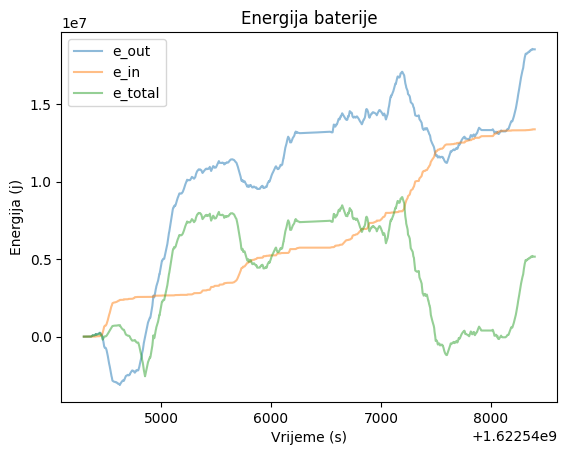
\includegraphics[width=0.8\textwidth]{images/energies_battery.png}
    \caption{Prikaz izračunate energije na bateriji kroz vrijeme.}
    \label{fig:h:energy_graph}
\end{figure}


\begin{table}[!ht]
    \centering
    \caption{Analiza energija na bateriji}
    \begin{tabular}{llll}
    \hline
        \textbf{describe} & \textbf{e\_out} & \textbf{e\_in} & \textbf{e\_total} \\ \hline
        """count""" & 9776.0 & 9776.0 & 9776.0 \\ 
        """null\_count""" & 0.0 & 0.0 & 0.0 \\ 
        """mean""" & 1.0358e7 & 6.5428e6 & 4.1977e6 \\ 
        """std""" & 5.4191e6 & 3.9817e6 & 3.4035e6 \\ 
        """min""" & -3.1183e6 & 0.0 & -2.5612e6 \\ 
        """25\%""" & 9.7020e6 & 3.2059e6 & 357062.111733 \\ 
        """50\%""" & 1.2458e7 & 5.7457e6 & 5.1647e6 \\ 
        """75\%""" & 1.3339e7 & 9.5036e6 & 7.4284e6 \\ 
        """max""" & 1.8580e7 & 1.3388e7 & 9.0084e6 \\ \hline
    \end{tabular}
    \label{table:c:energies_battery}
\end{table}